\newpage
\section{Resultados}
	\subsection{Histograma}
		O cálculo do histograma é um procedimento simples, onde um vetor que contém a intensidade (luminância)  de cada pixel é indexado pelo valor do mesmo e incrementado a cada pixel.
		
		\begin{figure}[!htb]
			\centering
			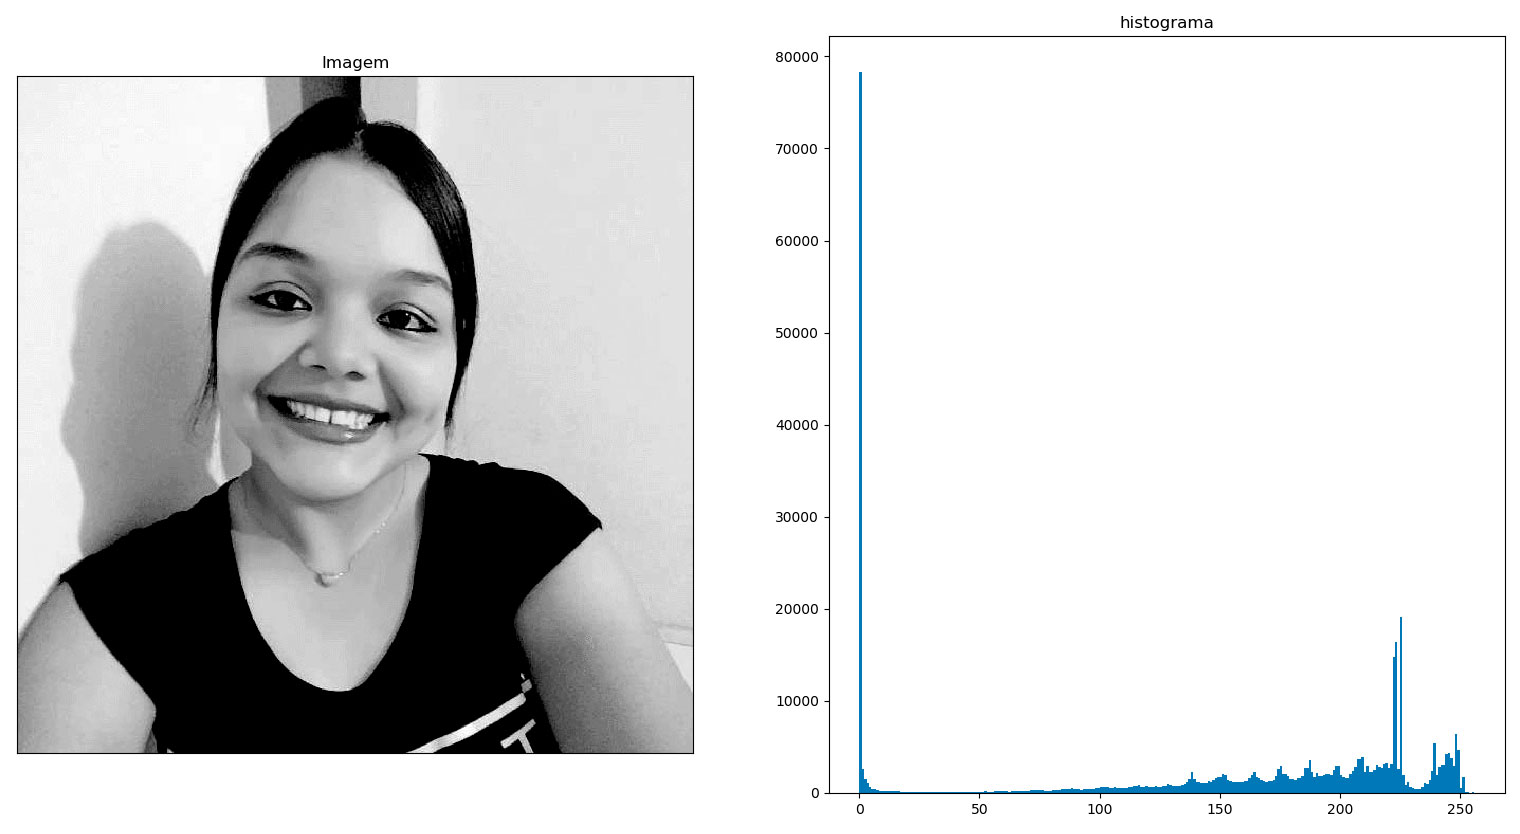
\includegraphics[width=\textwidth]{img/01-hist.jpg}
			\caption{Histograma da imagem}
		\end{figure}
	
		\lstset{language=c++}
		{\tiny \lstinputlisting{code/01-hist.cpp}}
		
	\subsection{Equalização do Histograma}
		O cálculo do histograma é um procedimento simples, onde um vetor que contém a intensidade (luminância)  de cada pixel é indexado pelo valor do mesmo e incrementado a cada pixel.
		
		\begin{figure}[!htb]
			\centering
			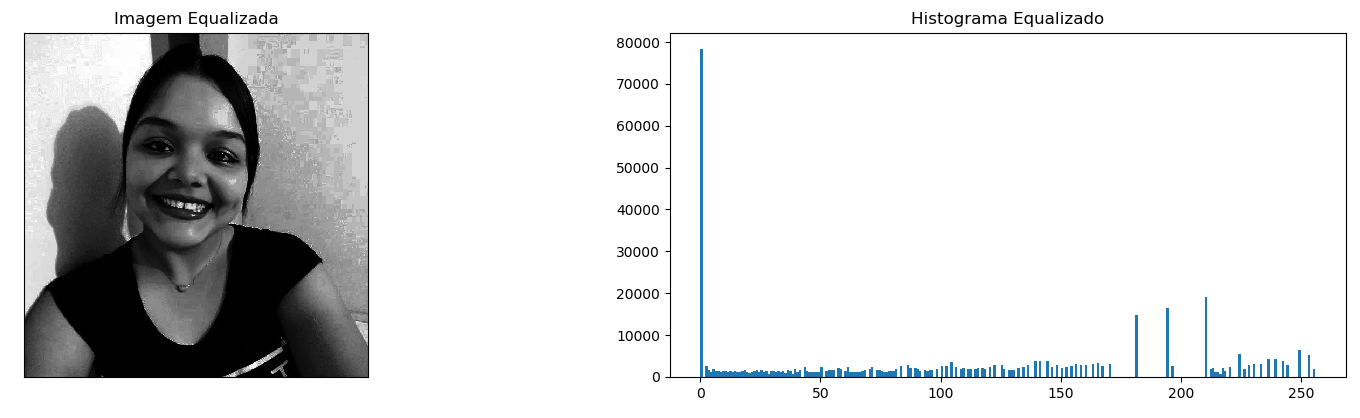
\includegraphics[width=\textwidth]{img/02-eq-hist.png}
			\caption{Histograma equalizado}
		\end{figure}
		
		\lstset{language=c++}
		{\tiny \lstinputlisting{code/02-eq-hist.cpp}}
		
	\subsection{Conversão para escala cinza}
		Algoritmo de escala de cinza baseado na luminosidade do pixel pela visão humana usando a fórmula: \texttt{L = R*0.3 + B*0.59 + G*0.11}. Dado o resultado o algoritmo salva o pixel na forma LLL. Primeiro convertemos a imagem em JPEG para PPM (formato simples e sem compressão, sendo mais fácil a manipulação), então obtemos um buffer dos pixels, na classe Image.
		
		\begin{figure}[!htb]
			\centering
			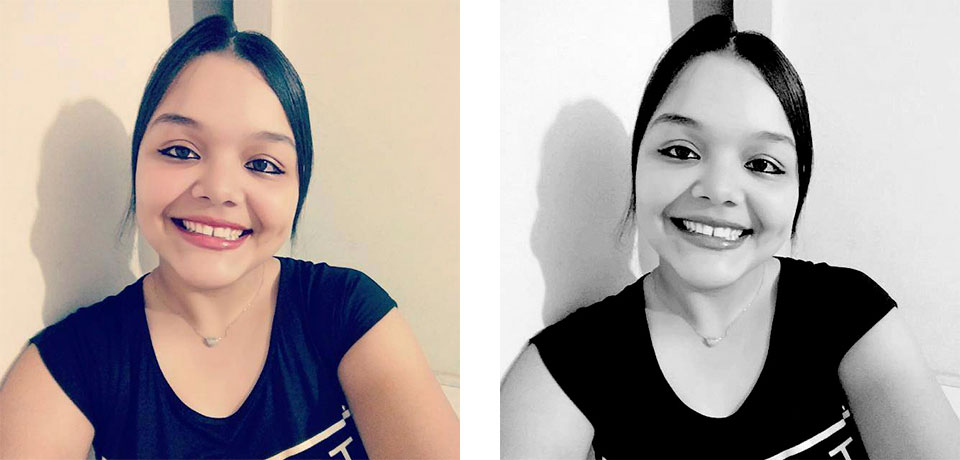
\includegraphics[width=\textwidth]{img/03-cinza.jpg}
			\caption{Imagem convertida para escala cinza}
		\end{figure}
		
		\lstset{language=Python}
		{\tiny \lstinputlisting{code/03-cinza.py}}
		
		\subsection{Rotacionamento de imagens}
			O método de rotação consiste em usar a matriz de pixel e deslocá-las de lugar como na imagem abaixo praticamente especificado.
			
			\begin{figure}[!htb]
				\centering
				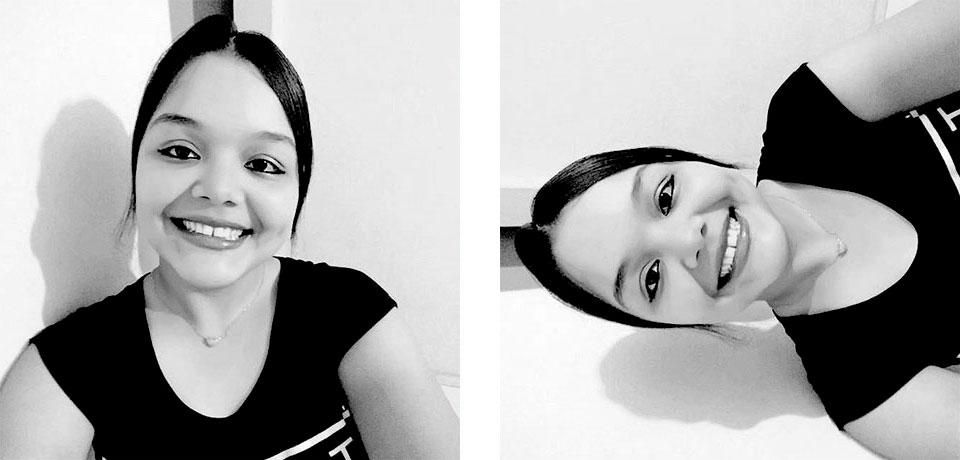
\includegraphics[width=\textwidth]{img/04-rotacao-1.jpg}
				\caption{Imagem rotacionada em sentido anti-horário}
			\end{figure}
			
			\begin{figure}[!htb]
					\centering
					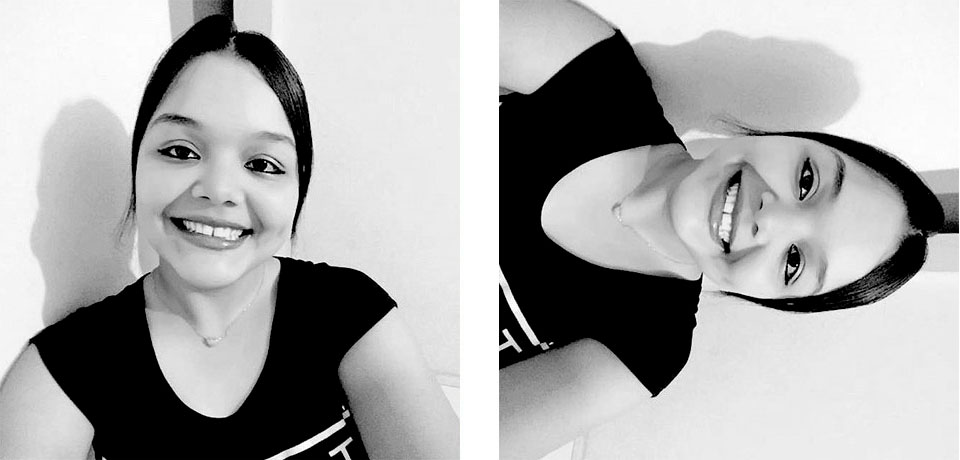
\includegraphics[width=\textwidth]{img/04-rotacao-2.jpg}
					\caption{Imagem rotacionada em sentido horário}
			\end{figure}
	
			\lstset{language=Python}
			{\tiny \lstinputlisting{code/04-rotacao.py}}
			
	\subsection{Redimensionamento}
		Ao dimensionar uma imagem gráfica, as primitivas gráficas que compõem a imagem podem ser dimensionadas usando transformações geométricas, sem perda de qualidade de imagem. Ao dimensionar uma imagem gráfica pixelada, uma nova imagem com um número maior ou menor de pixels deve ser gerada.
		No caso de diminuir o número de pixels (redução de escala), isso geralmente resulta em uma perda de qualidade visível. Do ponto de vista do processamento de sinal digital , o dimensionamento de gráficos de varredura é um exemplo bidimensional de conversão de taxa de amostragem, a conversão de um sinal discreto de uma taxa de amostragem (neste caso, a taxa de amostragem local) para outra.
		
		Há vários algoritmos para se fazer esse processo, alguns deles são: 
		\begin{itemize}
			\item Interpolação de vizinhança mais próxima
			\item Algoritmos bilineais e bicúbicos
			\item Reaprovação Sinc e Lanczos
			\item Amostragem de caixa
			\item Mipmap
			\item Métodos de transformada de Fourier
			\item Interpolação dirigida por borda
			\item HQX
			\item Vetorização			
		\end{itemize}
		
		\begin{figure}[!htb]
			\centering
			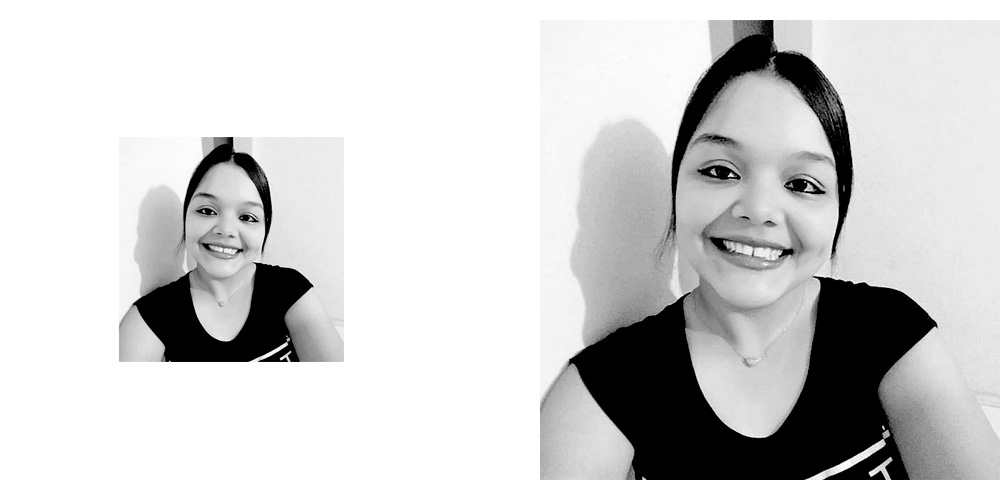
\includegraphics[width=\textwidth]{img/05-redimen.jpg}
			\caption{Imagem redimensionada}
		\end{figure}
		
		\lstset{language=Python}
		{\tiny \lstinputlisting{code/05-redimen.py}}
		
	\subsection{Espelhamento}
		O espelhamento da imagem é a inversão dos pixel na matriz no sentido oposto, por exemplo, um espelhamento horizontal os pixel da direita são movidos para a esqueda e, no espelhamento vertical os pixels inferiores são movidos para cima. 
		
		\begin{figure}[!htb]
			\centering
			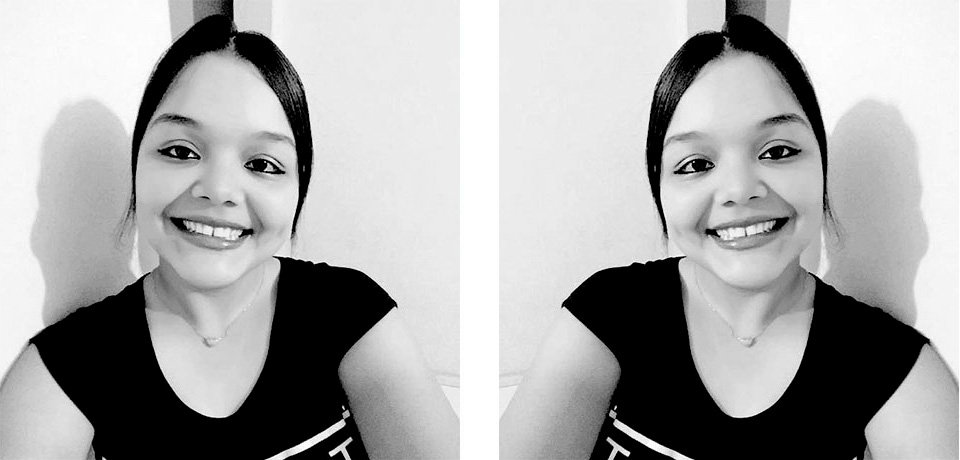
\includegraphics[width=\textwidth]{img/06-espelho.jpg}
			\caption{Imagem espelhada horizontalmente}
		\end{figure}
		
		\lstset{language=c++}
		{\tiny \lstinputlisting{code/06-espelho.cpp}}
		
		\begin{figure}[!htb]
			\centering
			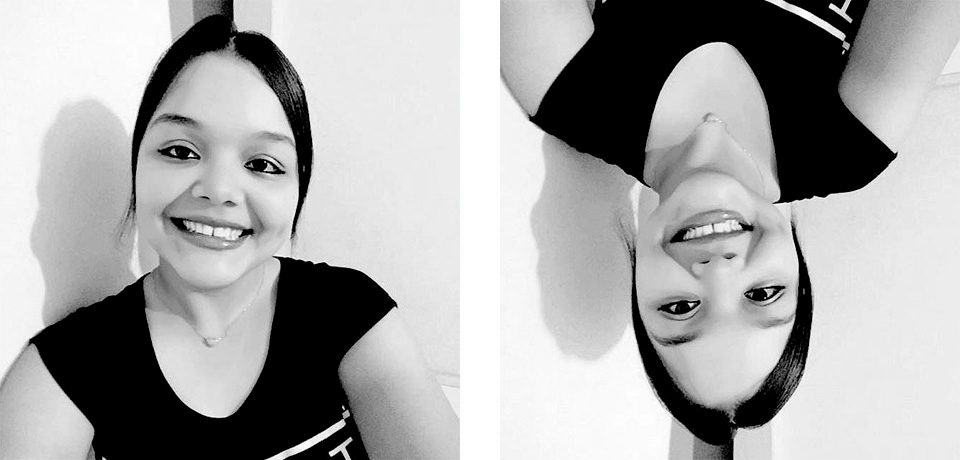
\includegraphics[width=\textwidth]{img/06-espelho2.jpg}
			\caption{Imagem espelhada verticalmente}
		\end{figure}
		
		\lstset{language=c++}
		{\tiny \lstinputlisting{code/06-espelho2.cpp}}
		
	\subsection{Negativo}
		Para se gerar uma imagem negativa é necessário efetuar os seguintes passos:
		
		\begin{enumerate}
			\item Extrair o fator de luminância da imagem para a cor cinza
			\item criar uma nova cor utilizando para os valores de RGB o fator de escala de cinza obtido
		\end{enumerate}

		No caso, esta luminância em cinza é baseada em 30\% de vermelho, 59\% de verde e 11\% de azul. Vale lembrar que como estamos trabalhando no padrão RGB o valor mínimo de uma cor é zero e o máximo e 255. Para realizar esta mudança em cada um dos pixels da imagem devemos percorrer todos os pixels da mesma, extrair a cor, gerar o fator de luminância para o cinza e alterar a cor do pixel.

		\begin{figure}[!htb]
			\centering
			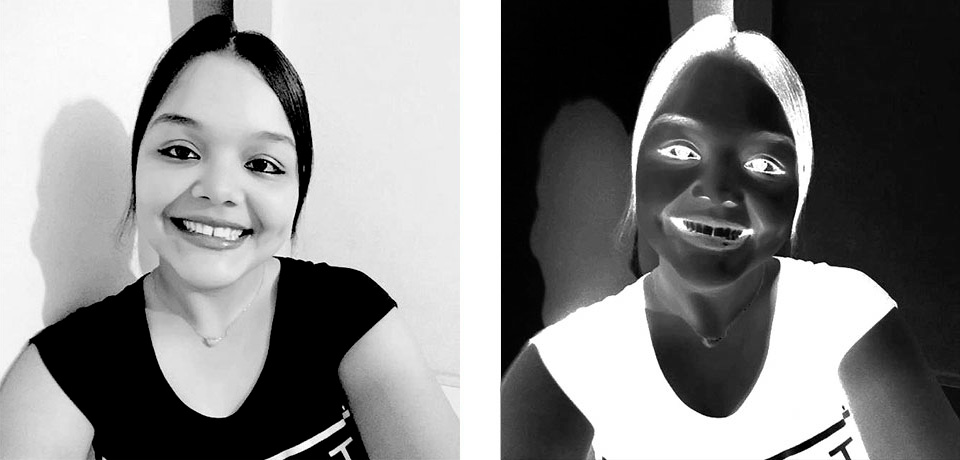
\includegraphics[width=\textwidth]{img/07-negativo.jpg}
			\caption{Imagem negativa}
		\end{figure}
		
		\lstset{language=c++}
		{\tiny \lstinputlisting{code/07-negativo.cpp}}
		
	\subsection{Brilho}
		Semelhantemente ao brilho, o contraste foi implementado usando-se um spin box para uma melhor precisão. O código implementado foi o seguinte:
		
		\begin{figure}[!htb]
			\centering
			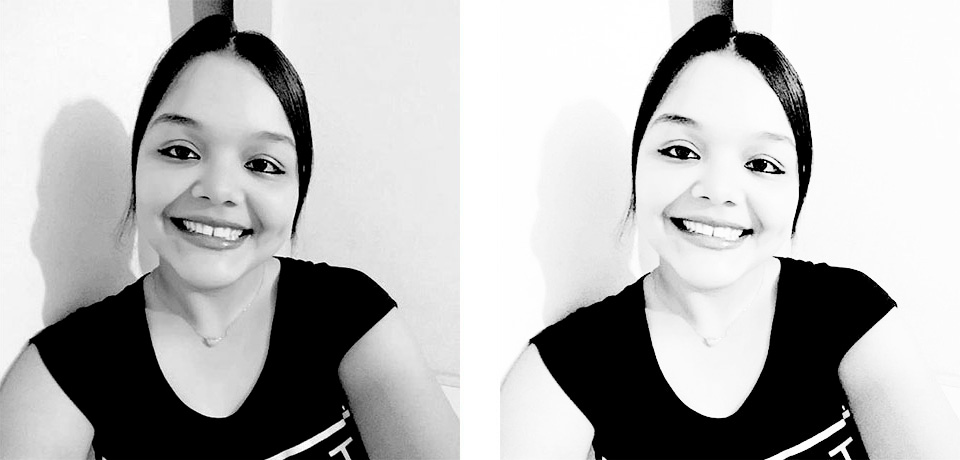
\includegraphics[width=\textwidth]{img/08-brilho.jpg}
			\caption{Imagem com brilho}
		\end{figure}
	
		\lstset{language=c++}
		{\tiny \lstinputlisting{code/08-brilho.cpp}}
		
	\subsection{Contraste}
		O ajuste de brilho é implementado como uma operação pixel a pixel usando-se uma função. Como foi utilizada uma slide bar, o procedimento usado foi salvar o estado anterior da slide bar para incrementar ou decrementar a variação da barra. A rotina para tratamento de cada mudança de valor na slide bar é a seguinte:
		
		\begin{figure}[!htb]
			\centering
			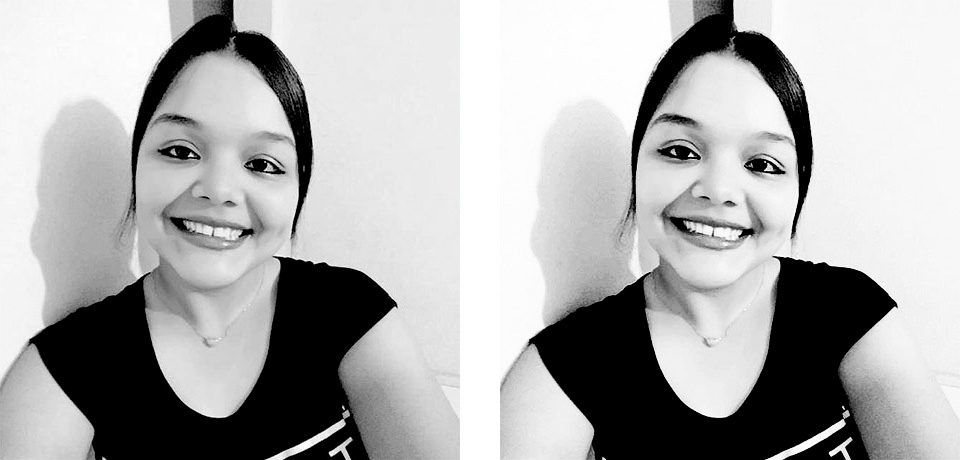
\includegraphics[width=\textwidth]{img/09-contraste.jpg}
			\caption{Imagem com contraste}
		\end{figure}
		
		\lstset{language=c++}
		{\tiny \lstinputlisting{code/09-contraste.cpp}}
	
	\subsection{Filtro Sobel}
		Consiste num operador que calcula diferenças finitas, dando uma aproximação do gradiente da intensidade dos pixels da imagem. Em cada ponto da imagem, o resultado da aplicação do filtro Sobel devolve o gradiente ou a norma deste vector, aplicada sobretudo em algoritmos de detecção de contornos.
		
		O filtro Sobel calcula o gradiente da intensidade da imagem em cada ponto, dando a direcção da maior variação de claro para escuro e a quantidade de variação nessa direcção. Assim, obtém-se uma noção de como varia a luminosidade em cada ponto, de forma mais suave ou abrupta.
		
		Com isto consegue-se estimar a presença de uma transição claro-escuro e de qual a orientação desta. Como as variações claro-escuro intensas correspondem a fronteiras bem definidas entre objectos, consegue-se fazer a detecção de contornos.
	
		\begin{figure}[!htb]
			\centering
			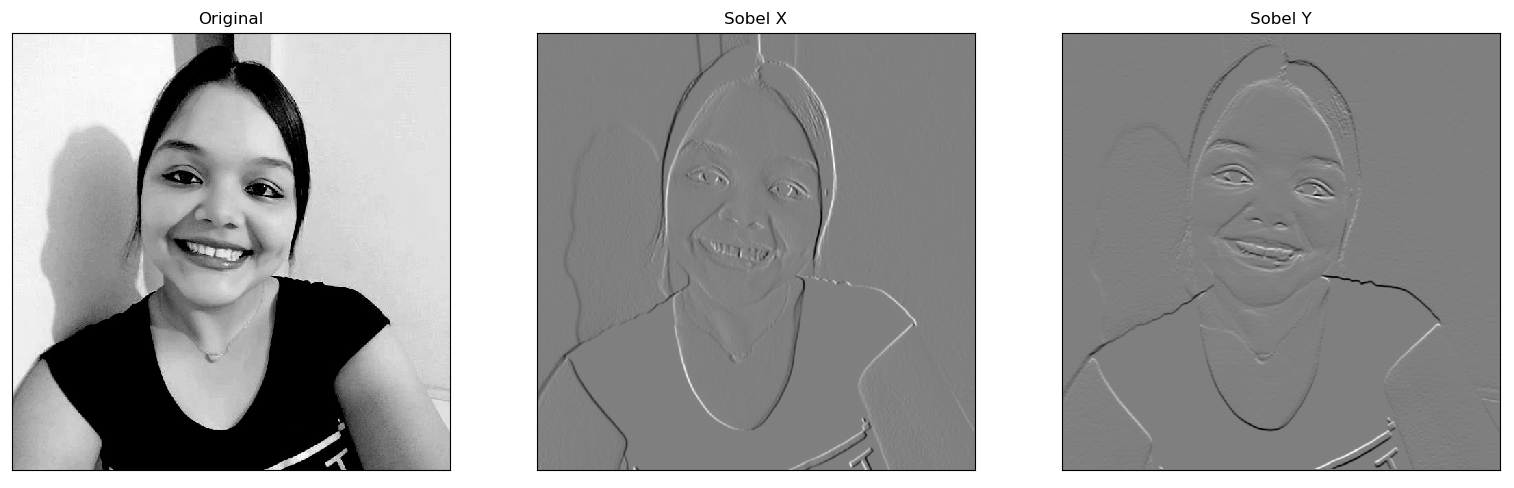
\includegraphics[width=\textwidth]{img/10-sobel.png}
			\caption{Filtro Sobel}
		\end{figure}
		
		\lstset{language=python}
		{\tiny \lstinputlisting{code/10-sobel.py}}
	
	\subsection{Filtro Prewitt}
		Em termos simples, o operador calcula o gradiente da intensidade da imagem em cada ponto, dando a direção do maior aumento possível da luz para a escuridão e a taxa de mudança nessa direção. O resultado, portanto, mostra como "abruptamente" ou "suavemente" a imagem muda nesse ponto e, portanto, como é provável que essa parte da imagem represente uma vantagem , bem como a forma como essa borda provavelmente estará orientada. Na prática, o cálculo da magnitude (probabilidade de uma borda) é mais confiável e mais fácil de interpretar do que o cálculo da direção.
	
		\begin{figure}[!htb]
			\centering
			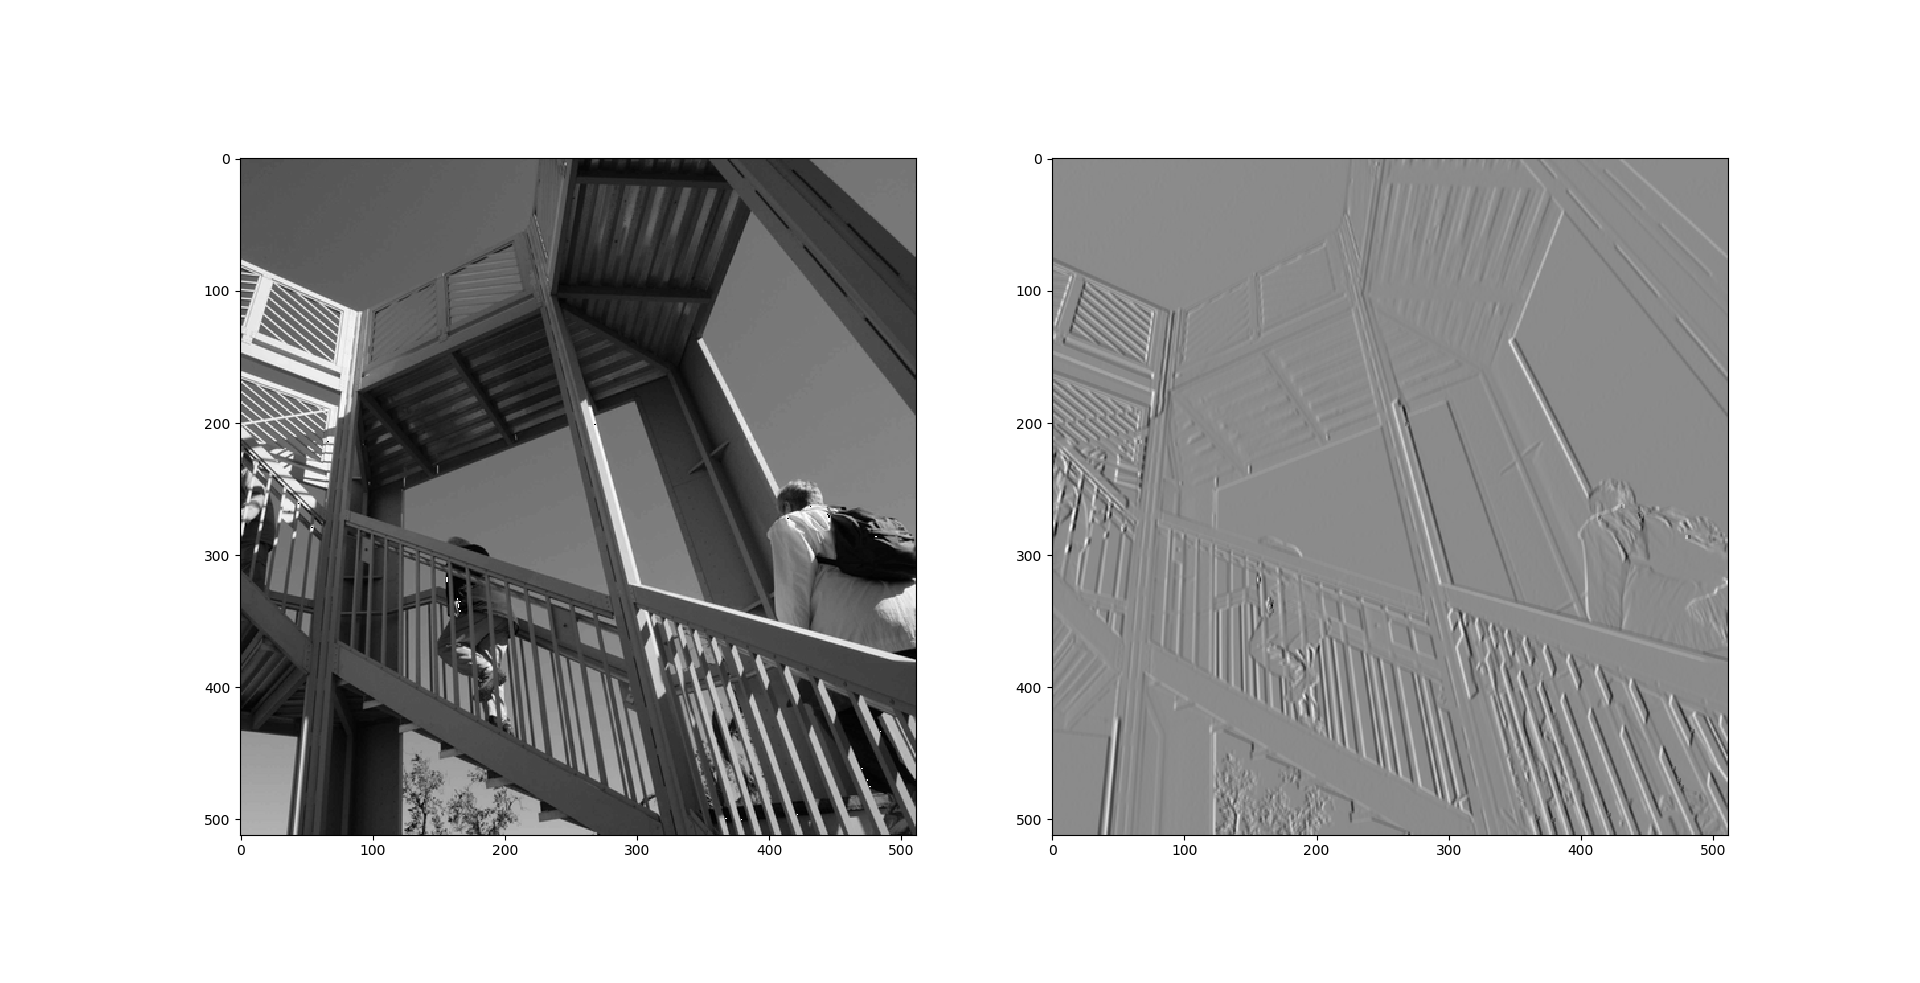
\includegraphics[width=\textwidth]{img/11-prewitt.png}
			\caption{Filtro Prewitt}
		\end{figure}
	
		\lstset{language=python}
		{\tiny \lstinputlisting{code/11-prewitt.cpp}}
		
	\subsection{Filtro Roberts}
		O operador Roberts cross é usado no processamento de imagens e visão computacional para detecção de borda. Foi um dos primeiros detectores de borda e foi inicialmente proposto por Lawrence Roberts em 1963. Como operador diferencial, a idéia por trás do operador Roberts Cross é aproximar o gradiente de uma imagem através de diferenciação discreta \textit{m} que é conseguida pela computação a soma dos quadrados das diferenças entre pixels diagonalmente adjacentes.

		\begin{figure}[!htb]
			\centering
			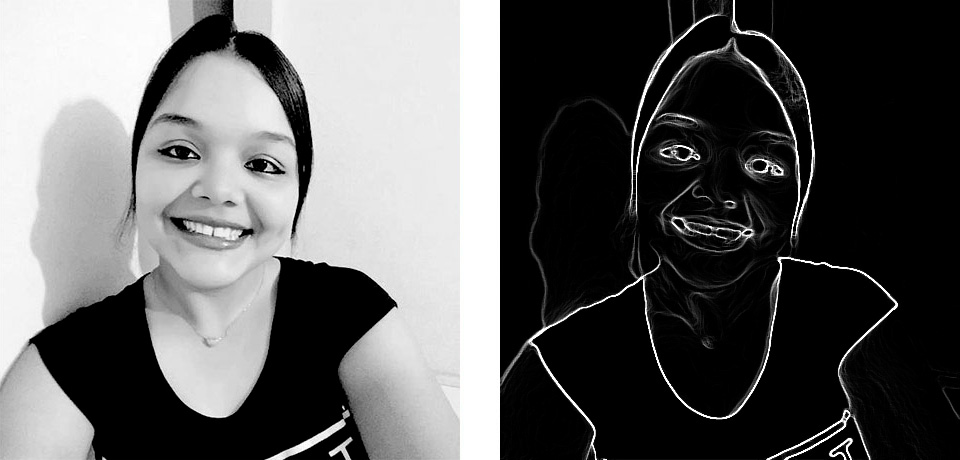
\includegraphics[width=\textwidth]{img/12-roberts.jpg}
			\caption{Filtro Roberts}
		\end{figure}
		
		\lstset{language=python}
		{\tiny \lstinputlisting{code/12-roberts.cpp}}
	
	\subsection{Filtro Canny}
		Desenvolvido por John F. Canny em 1986 o detector de bordas de Canny utiliza um algoritmo multi-estágios para detectar uma ampla margem de bordas na imagem. Canny também desenvolveu uma teoria computacional sobre detecção de bordas explicando porque as técnicas funcionam.
		John Canny propôs que o detector de bordas ótimo deveria respeitar os seguintes parâmetros:
		
		\begin{description}
			\item \textbf{Boa detecção}: O algoritmo deve ser capaz de identificar todas as bordas possíveis na imagem
			\item \textbf{Boa Localização}: As bordas encontradas devem estar o mais próximo possível das bordas da imagem original.
			\item \textbf{Resposta Mínima}: Cada borda da imagem deve ser marcada apenas uma vez. O ruído da imagem não deve criar falsas bordas.
		\end{description}

		Para satisfazer tais condições, Canny utilizou um cálculo de variações, visando encontrar uma função que otimizasse o funcional desejado. A função ideal para o detector de Canny é descrito pela soma de quatro termos de exponenciais, que pode ser aproximada pela primeira derivada de uma gaussiana.
		
		\begin{figure}[!htb]
			\centering
			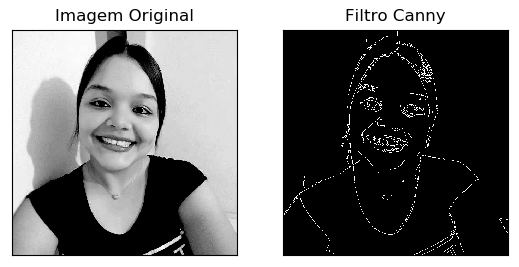
\includegraphics[width=\textwidth]{img/13-canny.png}
			\caption{Filtro Canny}
		\end{figure}
		
		\lstset{language=c++}
		{\tiny \lstinputlisting{code/13-canny.cpp}}
		
	\subsection{Filtro Laplaciano}
		É um filtro de detecção de bordas que gera uma borda fina de apenas um pixel de largura e é baseado numa derivada de 2ª ordem.
		
		\begin{figure}[!htb]
			\centering
			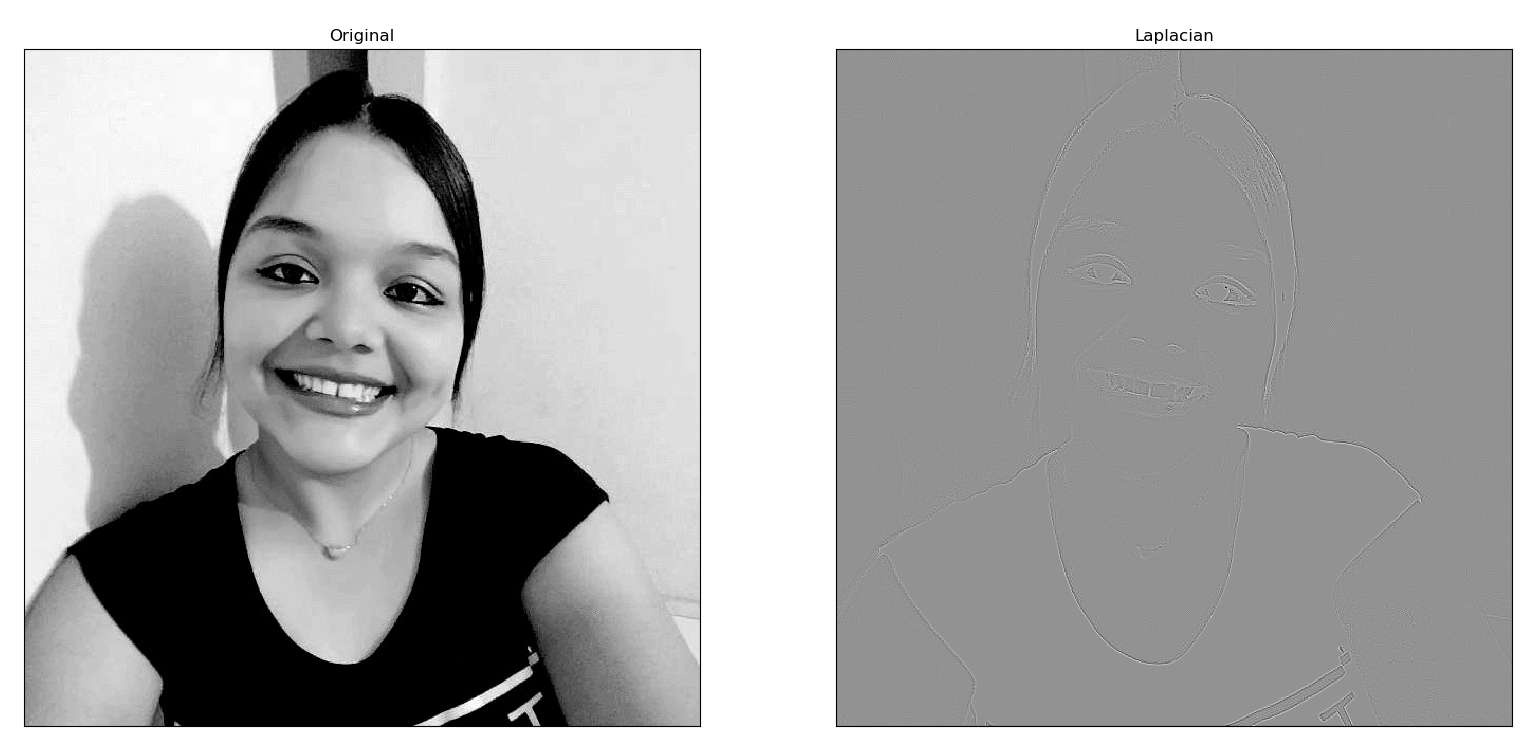
\includegraphics[width=\textwidth]{img/14-laplaciano.png}
			\caption{Filtro laplaciano}
		\end{figure}
	
		\lstset{language=c++}
		{\tiny \lstinputlisting{code/14-laplaciano.cpp}}
	
	\subsection{Filtro Média}
		Substitui o valor do pixel original pela média aritmética do pixel dos seus vizinhos. Quanto maior a máscara, maior o efeito de borramento. Pesos positivos. Soma dos pesos igual a 1 – não altera a média.
		
		\begin{figure}[!htb]
			\centering
			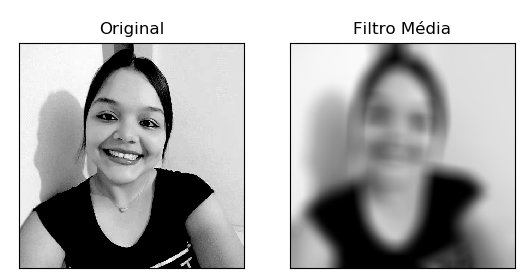
\includegraphics[width=\columnwidth]{img/15-media.png}
			\caption{Filtro Média}
		\end{figure}
		
		\lstset{language=c++}
		{\tiny \lstinputlisting{code/15-media.py}}
	
	\subsection{Filtro Mediana}
		Suaviza a imagem sem contudo diminuir sua resolução. os pontos da vizinhança de (x,y), dentro de uma janela na imagem, são ordenados e tomado como novo valor para (x,y) o valor mediano desta ordenação.
		
		\begin{figure}[!htb]
			\centering
			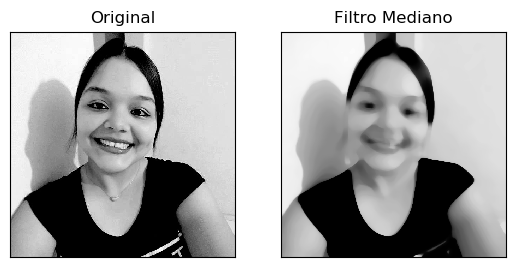
\includegraphics[width=\columnwidth]{img/16-mediana.png}
			\caption{Filtro Mediana}
		\end{figure}
		
		\lstset{language=python}
		{\tiny \lstinputlisting{code/17-mediana.py}}
		
	\subsection{Moda}
		Este filtro é usado para homogeneizar imagens temáticas, ou para reduzir ruídos mantendo o máximo de informação na imagem.
		
		\begin{figure}[!htb]
			\centering
			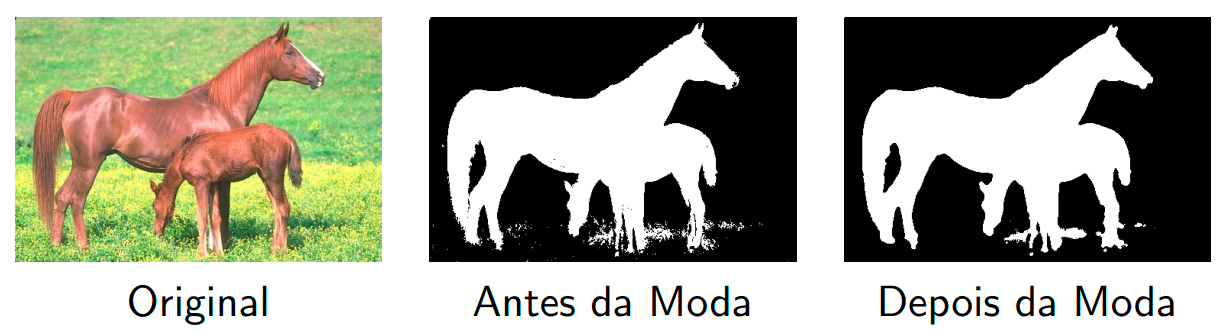
\includegraphics[width=\columnwidth]{img/18-moda.jpg}
			\caption{Filtro Moda}
		\end{figure}
		
	\subsection{Filtro Gaussiano}
		Um filtro gaussiano é utilizado para borrar ou desfocar a imagem na qual ele é aplicado com o objetivo de reduzir os ruídos presentes na imagem.  O resultado desta operação é a suavização da imagem, relembrando a visualização da mesma através de uma tela translúcida ou como se tivesse sendo vista através de uma lente fora de foco. A suavização gaussiana é largamente utilizada no estágio de pré-processamento da imagem a fim de enaltecer a estrutura da imagem em diferentes escalas.
		
		\begin{figure}[!htb]
			\centering
			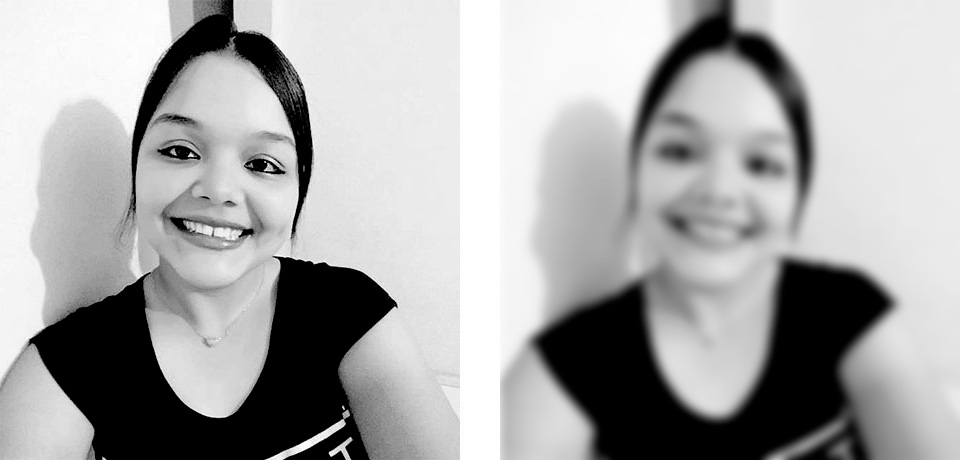
\includegraphics[width=\columnwidth]{img/19-gaussiano.jpg}
			\caption{Filtro Gaussiano}
		\end{figure}
		
		\lstset{language=python}
		{\tiny \lstinputlisting{code/19-gaussiano.java}}
		
		
		